\documentclass[11pt]{article}
\usepackage{a4,caption,listings,graphicx,enumerate,amsmath,amssymb,mathtools,lipsum,graphicx,microtype,float,xcolor, multicol, caption, fancyhdr, fourier-orns, datetime}
\usepackage[a4paper,margin=1in,footskip=0.25in]{geometry}
\usepackage[rightcaption]{sidecap}
\usepackage[sorting=none]{biblatex}


\title{\line(1,0){450} \\ \Huge\textbf{Insights through asymptotics:}\\
 \LARGE Benchmarking and analysis of climate effects on flood models}
\author{Henry Writer }

\newdateformat{monthyeardate}{%
  \monthname[\THEMONTH], \THEYEAR}

\date{\monthyeardate\today}

\usepackage{titlesec}
\renewcommand{\thesection}{\Roman{section}}

 
\titleformat{\section}[block]{\LARGE\bfseries\filcenter\titlerule\vspace{2mm}}{\thesection}{1em}{}

\titleformat{\subsection}[block]{\Large\bfseries\filcenter}{}{1em}{}
\pagestyle{fancy}
\fancyhead{}
\fancyhead[L]{Insights through asymptotics}
\fancyhead[R]{IIT-17 People and planet health}

\fancyfoot{}
\fancyfoot[C]{\thepage}
\fancyfoot[L]{Henry Writer}
\fancyfoot[R]{\monthyeardate\today}


\addbibresource{refs.bib}


\begin{document}

\maketitle

\section{Background}

There is currently unmistakable evidence that the climate of the planet is changing. We currently have a limited understand of what the potential outcomes of these changes may be. One route we have to understand these changes takes the form of mthamtical models, these then can be used to help us predict the future impact of climate change.

In the United Kingdom one of the largest potential effects of climate change we will encounter takes the form of river flooding. The government estimate that the cost of the 2015/16 floods is approximately 1.6 billion pounds. This number does not take into account the human toll of this event. 


Additionally, it appears that the number and severity of flooding is increasing. This has motivated the hydrological community in increasing the understanding of river flooding. This has been done by developing a `zoo' of potential flooding models. However, there are two problems regarding this large group of models, firstly since there is so many it is hard to separate them to decided which would be the most appropriate \cite{neelz2013benchmarking}. 
Secondly there is still information which is not being extracted from these models that can help us predict how flooding will change. We believe that we can solve both of these problems by examining models using asymptotic analysis.


\subsection{How do we model river flooding}
There are currently three main approaches to building flooding model. We have statistical models this relies on using statistical method to fit models to data and use statistical models to make inferences about the future, this class of models is not a major focus of this project. 

The other two classes of models which we will focus are efforts on will be conceptual models, these rely on creating a set of states from which the quantity of interest can move between this is best represented by a Figure \ref{fig:conceptual}. 
The other modelling technique of interest we have physical models these take a continuing mechanics approach and set up a set of conservation laws and use these to drive a set PDE equations that can then be used to model the flooding event.



\subsection{Conceptual models}

 As briefly mentioned in the previous section conceptual models attempt to capture a complex system such as river flooding and simplify it down to a set of possible states/locations where a quantity of interest may reside in. Travel between these states is then governed by a simple mathematical expression. These models are then trained on a real life example to choose parameter that control the mathematical expressions.
 
 \begin{minipage}{0.5\textwidth}
    \begin{figure}[H]
        \centering
        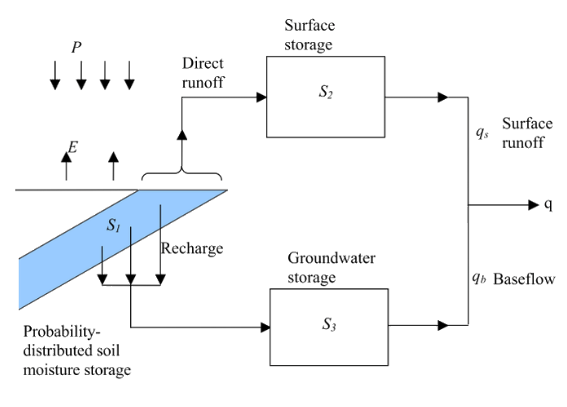
\includegraphics[width=0.6\textwidth]{Figs/Concept.png}
        \captionof{figure}{Example of a Conceptual model from \cite{https://doi.org/10.1002/joc.1539}}
        \label{fig:conceptual}
    \end{figure}
    \begin{figure}[H]
        \centering
        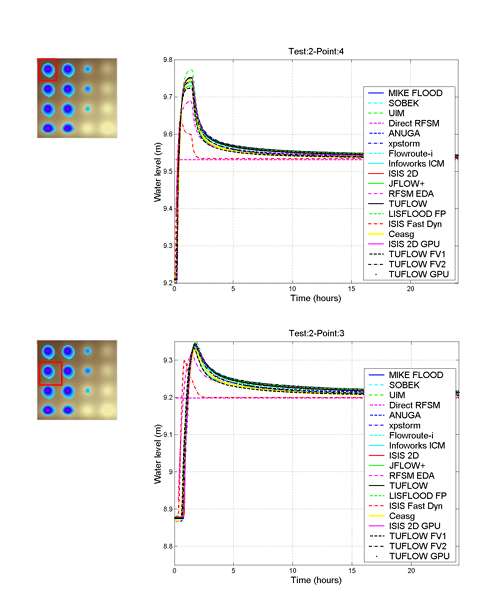
\includegraphics[width=0.6\textwidth]{Figs/EA_bench.png}
        \captionof{figure}{This demonstrate the challenges with separating different flooding models from each other. This figure is from \cite{neelz2013benchmarking}}
        \label{fig:eaBench}
    \end{figure}
\end{minipage}
\hspace{0.05\textwidth}
\begin{minipage}{0.4\textwidth}
    \qquad Figure \ref{fig:conceptual} gives a diagrammatic example of a conceptual model this model show how rain water might flow through a catchment area. It shows rain entering the system via precipitation and then the path it might take, either evaporating immediately, or by flowing into surface or groundwater storage, before being eventually discharged into a stream.

    \qquad We can see that conceptual modelling allow us to easily build a model that in can incorporate many aspects of a system. However, with how relatively simple it is to designing these models means that there is a `zoo' of similar models from which we could use to model a potential river catchment area. This issue of benchmarking these models to determine which one is mots suitable for a given situation are discussed in \cite{neelz2013benchmarking}. 
    Figure \ref{fig:eaBench}  graphically demonstrates the challenge posed in differentiating flooding models. This is one of the major motivations of the proposed asymptotic benchmarking process.
\end{minipage}



\subsection{How do we currently interpret the output of flooding models}

\begin{minipage}{0.35\textwidth}
    Another motivation to creating a methodology to derive scaling laws from conceptual models is in the predication of future flooding events. 
    The method currently used to give predictions of future flooding evolves taking a handful of different data sets that model a potential climate under a variety of possible climate scenarios. These data sets are then feed in to a conceptual model then these outcomes are used to draw inferences about future floods.
    This process can be visualised in the flow diagram in Figure \ref{fig:flow}.
\end{minipage}
\hspace{0.05\textwidth}
\begin{minipage}{0.55\textwidth}
    \begin{figure}[H]
    \centering
    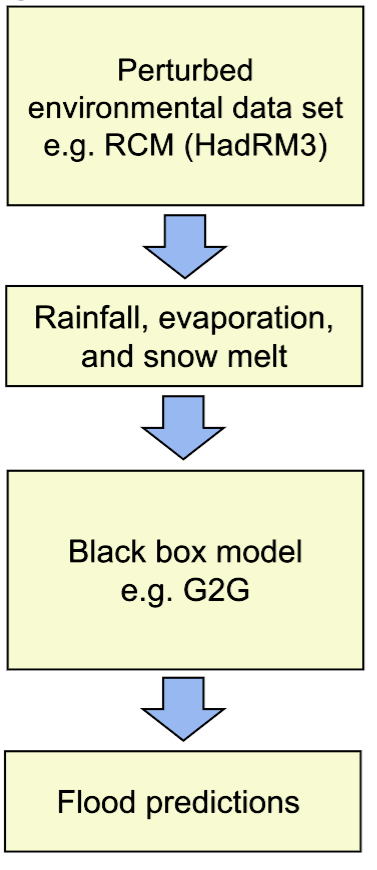
\includegraphics[width=0.25\textwidth]{Figs/flow.png}
    \captionof{figure}{Flow chart demonstrate the way in which outcomes of climate change are used to give estimat}
    \label{fig:flow}
\end{figure}
\end{minipage}

\vspace{5pt}

The paper \cite{BELL201289} is a good reference for how this process is carried out in practice. Figure \ref{fig:concept_in} shows the different rainfall data that is then entered in to the model, and Figure\ref{fig:concept_out} show the output form there model. They then use the output form these models to make simple predictions about the effect of climate change.

We think that our asymptotic benchmarking process that we can do better by deriving psychical scaling laws that will can give additional insight in to how flooding events will scale with different environmental conditions.

\begin{minipage}{0.6\textwidth}
    \begin{figure}[H]
    \centering
    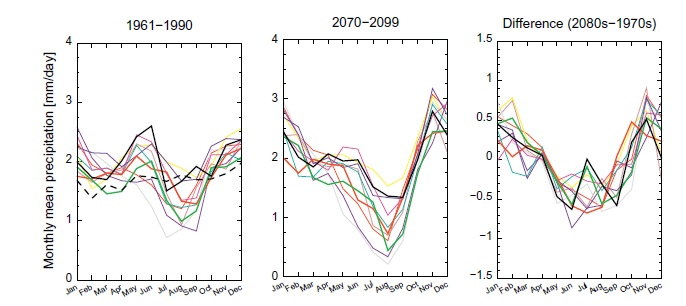
\includegraphics[width=\textwidth]{Figs/concept_in.jpg}
    \captionof{figure}{Shows how the different data sets change the rainfall which is entered in the flooding model. This figure is taken from~\cite{BELL201289}.}
    \label{fig:concept_in}
\end{figure}
\end{minipage}
\hspace{0.05\textwidth}
\begin{minipage}{0.3\textwidth}
    
\begin{figure}[H]%this figure will be at the left
    \centering
    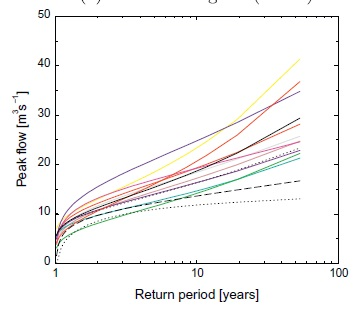
\includegraphics[width=\textwidth]{Figs/concept_out.jpg}
    \captionof{figure}{Show the effect of the different rainfalls on the outcomes on the model. This figure is taken from~\cite{BELL201289}.}
    \label{fig:concept_out}
\end{figure}
\end{minipage}




\subsection{Reduced PDE model}
Another model of interest is a reduced PDE model. This model has been developed by a current SAMBa student Piotr as part of thesis. 
We believe that we can continue this work and develop this model further by using asymptotic methods.
We shall briefly outline how this model works, this brief exploration will omit many of the major details this can be found in the these papers~\cite{pp1},\cite{pp2} and~\cite{pp3}.

\vspace{5pt}
\begin{minipage}{0.6\textwidth}
    \begin{figure}[H]%this figure will be at the left
    \centering
    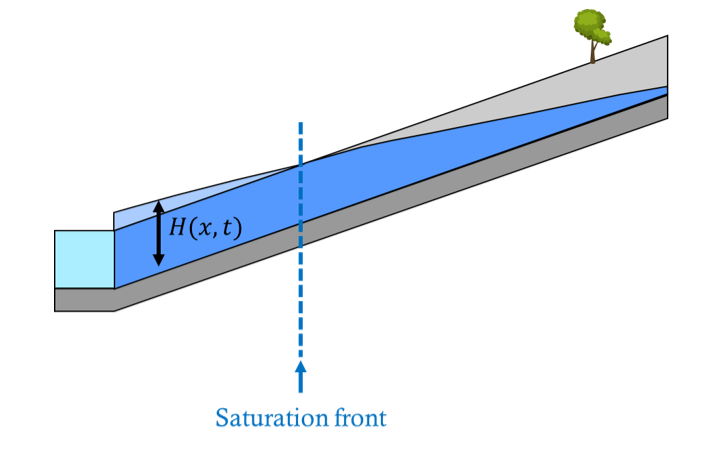
\includegraphics[width=\textwidth]{Figs/Simple model.png}
    \captionof{figure}{This plot gives a demonstrates how the PDE model works. This figure is form~\cite{pp2}}
    \label{fig:model}
    \end{figure}
\end{minipage}
\hspace{0.05\textwidth}
\begin{minipage}{0.3\textwidth}
    \qquad For this model to work we reduce the complexity of the river by assuming that it travel in a straight line, with the river laying at the bottom of a v shaped channel. Additionally, we assume there are two types of equation governing the behaviour of the flow of water toward the river. 
    The flow in the `unsaturated zone' this is where a flood has not started the water is contained below ground level. The other region the water travels through is the `saturated zone' this is the area where the soil has become saturated, and a flood has formed. The equation for this system is given below,
    
\end{minipage}

 \begin{align}
    H_t=\begin{cases}
        f(x)^{-1}[(\sigma HH_x+H)_x+p_0\times\text {rainflall}] \qquad \qquad  \ \; \text{in the unsaturated zone},\\
        (\sigma H_x+\mu\sqrt{1+\sigma H_x}(H-1)^{5/3})+p_0 +\text{rainfall} \quad \text{in the saturated zone}, \label{reduced PDE}
    \end{cases}
\end{align}

where $H(x,t)$ is the hight of the fluid at position $x$ and time $t$.


\section{Problem formulation and method}
The core of this program of work will take two forms. First we will develop this asymptotic benchmarking tool, and secondly we will explore extensions to the reduced PDE model. 
\subsection{A new approach to benchmarking}
As we discussed earlier there is work to be done in improving the insights which we can get from conceptual models. The plan will be to derive asymptotic scaling laws for these conceptual models. These laws will be able to tell us how some desired quantity is scaled based upon some input. So for example from the reduced PDE model (\ref{reduced PDE}) we would wish to develop a scaling law of the following form, $H(r(t))$, where $r(t)$ is some changing rainfall. 

\vspace{5pt}

\noindent\begin{minipage}{0.53\textwidth}
    \qquad However deriving the scaling laws directly from the underlying models is likely to be difficult. We will first approach the problem numerically, this numerical scaling law can then be used to derive the analytical scaling law.
    
    \qquad To demonstrate this procedure we will use the reduced PDE model. First we pick some rainfall function in this case we we chose, \begin{align}
        r = r_0\epsilon,
    \end{align}
    where $r_0$ is some baseline rainfall. So in Figure \ref{fig:S14_fig1} each colour of line represents a different value of alpha. Next we fix some time in this case we pick time such that the groudn is saturated and a flood has formed. 
    
    \qquad Next we then take these values of $H(r)$ and attempt to fit some function to them. In this case this can be seen in Figure \ref{fig:S14_fig2} which is loglog plot form this we get that $H(r)$ scales form some power law more precisely, \begin{align}
    H(r)=r_0^{\epsilon}.
    \end{align}
    
    \qquad We will confirm this by asymptotically examining the model, unfortunately during the preliminary investigations which we carried out during ITT17 we did not have time analytical derive the scaling law for this model.
    \end{minipage}
\hspace{0.05\textwidth}
\begin{minipage}{0.37\textwidth}
    \begin{figure}[H]%this figure will be at the left
    \centering
    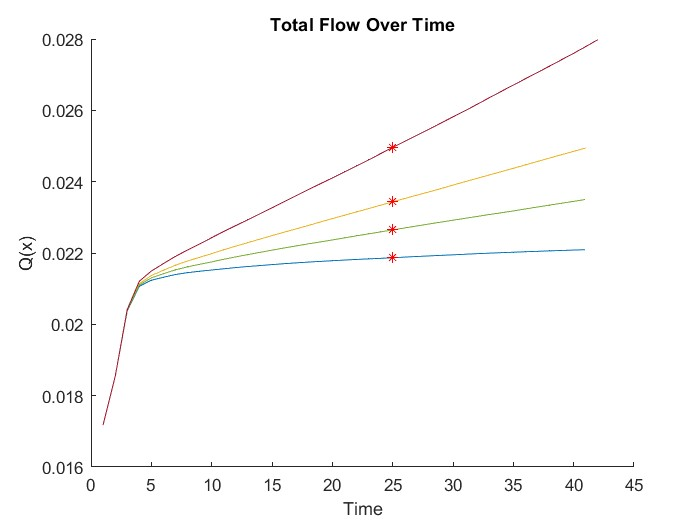
\includegraphics[width=\textwidth]{Figs/S14_fig1.jpg}
    \captionof{figure}{This figure shows how the $H(x,t)$ given different rainfall.}
    \label{fig:S14_fig1}
    \end{figure}
    \begin{figure}[H]%this figure will be at the left
    \centering
    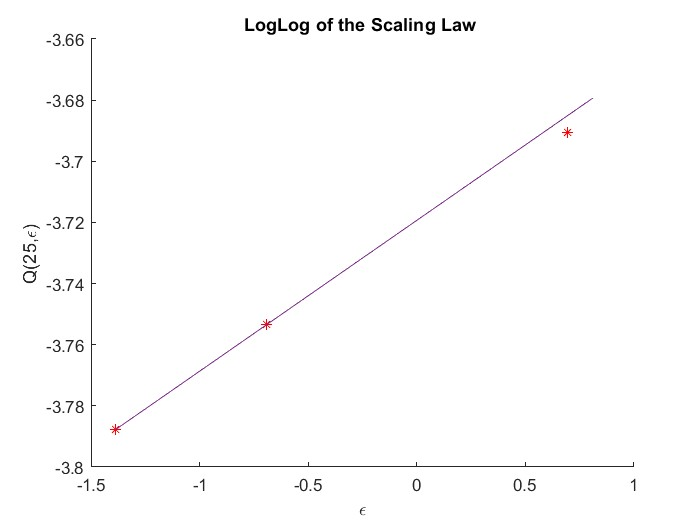
\includegraphics[width=\textwidth]{Figs/S14_fig2.jpg}
    \captionof{figure}{A loglog plot used to fit derive the numerical scaling law.}
    \label{fig:S14_fig2}
    \end{figure}
\end{minipage}

\vspace{5pt}

\qquad The two reasons why we wish to do numerical analysis first is that it will significantly speed up the search for analytically derived laws, we will be able to use the numerically derived law as a ansatz. Secondly there is scope to develop the numerical work flow into a R package that will allow industry to test there models quickly and independently.



\subsection{Extending the model with multiple time scales}

\begin{minipage}{0.45\textwidth}
    \begin{figure}[H]
    \centering
    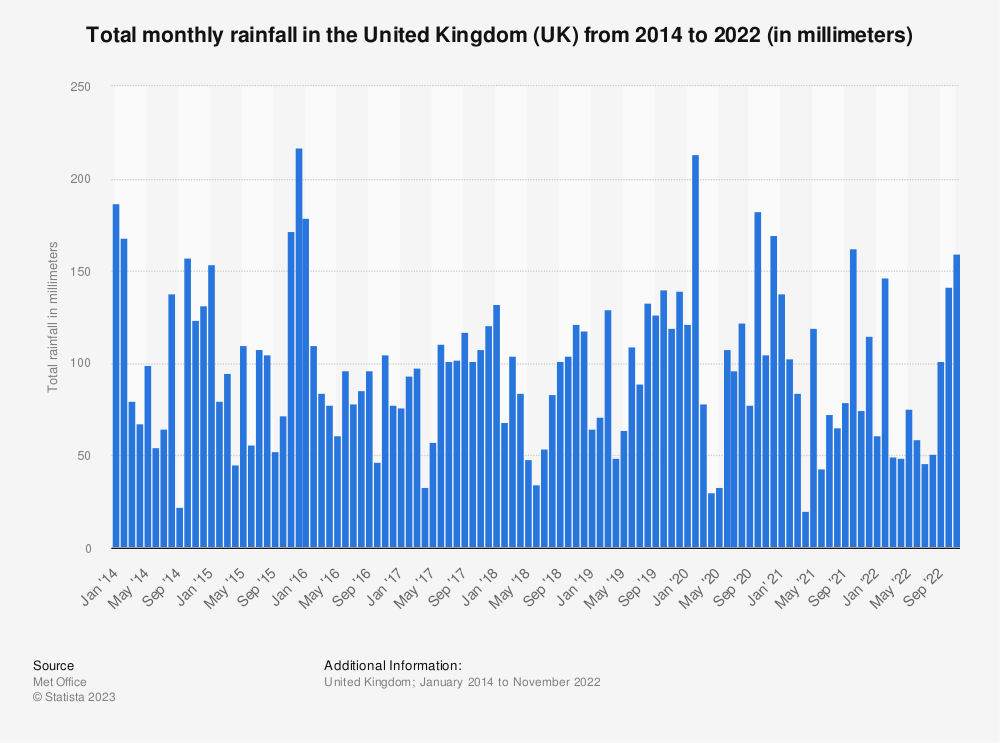
\includegraphics[width=\textwidth]{Figs/Rainfall.png}
    \captionof{figure}{Monthly rainfall data for the UK taken over a period 2024-2022 taken from the Met Office.}
    \label{fig:rainfall}
    \end{figure}
\end{minipage}
\hspace{0.05\textwidth}
\indent\begin{minipage}{0.45\textwidth}
    The second strand of the proposal will focus on extending the reduced PDE model to accommodate more complex forms of rainfall functions. Currently the model has only been explored with constant rainfall, this is clearly not hwo the weather acts in real world see Figure \ref{fig:rainfall} which is the monthly rainfall for the UK. 
    Clearly this rainfall is not constant and in fact appears to have behaviour working on some short time scale, the seasonal difference in rainfall, and behaviour working on some larger multiple year time scale.

    \qquad We should hopefully be able to explore this behaviour using the asymptotic method of multiple time scales to get more complex predictions from the model.
\end{minipage}

\vspace{5pt}
\subsection{People}
Below are the group of people who would make a the supervisory team for this project.
\begin{itemize}
    \item Primary supervisor: \textbf{Dr. Philipp Trinh}.
    \item Secondary supervisor: \textbf{Dr Lisa Kreusser}.
    \item External collaborator: \textbf{Professor Rob Lamb} with the JBA group.
\end{itemize}



\section{Objectives and strategy}

The work outlined above is designed to be undertaken as PhD project. A potential student undertaken this project would require a strong background in fluid mechanics, asymptotic analysis and, would require a passion for environmental mathematics. 
Additionally, it would be beneficial if a potential student had some experience with time series analysis, and numerical PDEs.

\subsection{Objectives}
Below is a list of initial targets which shall form the core of the project.

\begin{enumerate}
    \item \textbf{Numerical derive scaling laws,} from conceptual models. This would require first conducting a literature review to ascertain influential models that our benchmarking method could be applied to. Then apply the benchmarking process as outlined earlier to these models, to derive numerical scaling laws.
    \item \textbf{Analytically derive scaling laws,} this shall be accomplished by using numerical laws derived earlier to inform a exploration of the conceptual models.
    \item \textbf{Apply periodic rainfall to the reduced PDE model}. To this end we will need to conduct a time series analysis of rainfall data, from variety of source to allow us to work out appropriate rainfall functions and time scales to inform the analysis of the reduced PDE model.
\end{enumerate}

\subsection{Potential future objectives}

There are a number of directions this project may be extended dependent upon the interests of the student. A couple of potential avenues of extension are outlined below to show the scope of where this project mighty lead.

 The reduced PDE model has a number of other extension which can be explored. One approach would be to use the asymptotic method of homogenization, this would allow us to explore how a more complex soil structure how this will effect flooding events. Another approach we could use to examine the flow in soil would be to replace the equation which governs the flow through the soil with a equation that would allow us to explore channelling behaviour in the soil.

We could also take a dynamical systems approach to the analysis of the reduced PDE model. For example it is very natural to assume that there are two possible states in which a catchment area could be in, a saturated state this would be equivalent to a wetland, and a dry/drought state. We then assume that as the land dry out it becomes less porous so more water flows directs overland. We can then explore how much rainfall would have to change to transition between these states.

Another promising avenue we could explore would be in attempting to match the conceptual models with the reduced PDE model. This would be of great interest as the different methodologies for building flooding models are are currently some what isolated form each other. By matching the PDE model to a conceptual model we hope to be able to connect these model to gether and in the process gain more information about the different modelling techniques.

These three possible research direction are not meant to outline the scope of this project and its potential.



\section{Impact}
Like all research proposal we believe that we are carrying out novel and interesting mathematics. Additionally due to the subject of this research on climate change and namely river flooding which is one of a major extensional threat to the United Kingdom and the wider world. Any additional understanding of flooding mechanics and additional predictions will prove to be extremely valuable.
\subsection{Mathematical impact}
To emphasise the mathematical impact of this project here is a non-exhaustive list of the novel mathematics. 
\begin{itemize}
    \item Applying asymptotic methods to derive scaling laws form conceptual climate models is a potential new application for these methods.
    \item A deep analytical analysis of conceptual modelling methods we will help to give understanding of how these commonly used techniques will behaviour.
    \item The application of a multiple time scales analysis to the reduced PDE models is very likely to generate new and interesting problems which will need to be solved.
\end{itemize}

\subsection{Industrial impact}
As this problem has been brought forward by the Environments Agency there is a clear interest in this type of work from industry. But more concretely there is a very large motivation from practising hydrologists for a rigours analysis of the conceptual models that form a important of there practice. Additionally, we believe that the scaling laws that will be derived during this process may help to inform how we manage the risks of river flooding.

Finally, the second strand of this project in extending the PDE model to incorporate periodic forcing we will allow us to help examine seasonal rainfall and examine/predict changes in potential flooding over the timescale of climate change. This type of analysis is challenging for industry to carry out and is prime territory for a PhD project.




\printbibliography


\end{document}